%%%%%%%%%%%%%%%%%%%%%%%%%%%%%%%%%%%%%%%%%%%%%%%%%%%%%%%%%%%%%%%%%%%%%%%%
%    INSTITUTE OF PHYSICS PUBLISHING                                   %
%                                                                      %
%   `Preparing an article for publication in an Institute of Physics   %
%    Publishing journal using LaTeX'                                   %
%                                                                      %
%    LaTeX source code `ioplau2e.tex' used to generate `author         %
%    guidelines', the documentation explaining and demonstrating use   %
%    of the Institute of Physics Publishing LaTeX preprint files       %
%    `iopart.cls, iopart12.clo and iopart10.clo'.                      %
%                                                                      %
%    `ioplau2e.tex' itself uses LaTeX with `iopart.cls'                %
%                                                                      %
%%%%%%%%%%%%%%%%%%%%%%%%%%%%%%%%%%
%
%
% First we have a character check
%
% ! exclamation mark    " double quote
% # hash                ` opening quote (grave)
% & ampersand           ' closing quote (acute)
% $ dollar              % percent
% ( open parenthesis    ) close paren.
% - hyphen              = equals sign
% | vertical bar        ~ tilde
% @ at sign             _ underscore
% { open curly brace    } close curly
% [ open square         ] close square bracket
% + plus sign           ; semi-colon
% * asterisk            : colon
% < open angle bracket  > close angle
% , comma               . full stop
% ? question mark       / forward slash
% \ backslash           ^ circumflex
%
% ABCDEFGHIJKLMNOPQRSTUVWXYZ
% abcdefghijklmnopqrstuvwxyz
% 1234567890
%
%%%%%%%%%%%%%%%%%%%%%%%%%%%%%%%%%%%%%%%%%%%%%%%%%%%%%%%%%%%%%%%%%%%
%
\documentclass[12pt,a4paper,final]{iopart}
\newcommand{\gguide}{{\it Preparing graphics for IOP journals}}
%Uncomment next line if AMS fonts required
\usepackage{iopams}
\usepackage{graphicx}
\usepackage[breaklinks=true,colorlinks=true,linkcolor=blue,urlcolor=blue,citecolor=blue]{hyperref}
\usepackage{url}
\usepackage{caption}
%\usepackage{amsmath,amssymb,amsthm,amscd}
%\usepackage{natbib}

\usepackage[all]{xy}
\newcommand{\eq}{\mbox{eq}}
\newcommand{\dt}{\mathit{dt}}
\newcommand{\bbM}{\mathbb M}
\newcommand{\bt}{\pmb\theta}
\newcommand{\Bt}{\pmb\Theta}
\newcommand{\vc}[1]{{\bf #1 }}


\begin{document}

\title[Parameter inference with stochastic models]{Bayesian Parameter Inference for Nonlinear Stochastic Differential Equation Models}

\author[cor1]{Carlo Albert}%$^{1,2}$
\address{Eawag, Swiss Federal Institute of Aquatic Science and Technology, 8600 D\"ubendorf, Switzerland}
%\address{$^2$Address Two, Neverland}
\ead{carlo.albert@eawag.ch}

\author{Simone Ulzega}
\address{Eawag, Swiss Federal Institute of Aquatic Science and Technology, 8600 D\"ubendorf, Switzerland}
\ead{simone.ulzega@eawag.ch}

%\author[cor1]{Author Three}
%\address{Address Four, Neverland}
%\eads{\mailto{author.three@mail.com}, \mailto{author.three@gmail.com}}


\begin{abstract}
Bayesian statistics has become an indispensable tool in many applied sciences for the purpose of uncertainty analysis.
Inferring parametric uncertainty for stochastic differential equation (SDE) models, however, is a computationally hard problem due to the high dimensional integrals that have to be calculated.
Here we present a Monte Carlo-based method for Bayesian parameter inference with one dimensional SDE models to tackle the generic problems of calibrating the model to given data time series while simultaneously quantifying the ensuing parametric uncertainty.
%Here, we consider the generic problem of calibrating a one dimensional SDE model to %time series and quantifying the ensuing parametric uncertainty.
We re-interpret the Bayesian posterior distribution for model parameters as the partition function of a statistical mechanical system and employ a Hamiltonian Monte Carlo algorithm to calculate it.
Depending on the number of discretization points and the number of measurement points the dynamics of this system happen on very different time scales.
Thus, we employ a multiple time scale integration together with a suitable re-parametrization to derive an efficient inference algorithm.
While the algorithm is presented by means of a simple SDE model from hydrology, it is readily applicable to a wide range of inference problems. Furthermore the algorithm is highly parallelizable.

\end{abstract}

%Uncomment for PACS numbers title message
\pacs{00.00, 20.00, 42.10}
% Keywords required only for MST, PB, PMB, PM, JOA, JOB?
\vspace{2pc}
\noindent{\it Keywords}: Bayesian parameter inference, Hamiltonian Monte Carlo, time series analysis, stochastic differential equations

% Uncomment for Submitted to journal title message
\submitto{\NJP}
% Comment out if separate title page not required
%\maketitle

\section{Introduction}

Phenomenological models are employed in many applied areas of research to predict the behaviour of complex systems of all sorts.
Parameters of these models often don't have a direct physical meaning and need to be inferred from measurements.
In order to make reliable predictions with such models it is important to describe the dominant errors in the model and to quantify the parametric uncertainty resulting from the inference process.

{\em Bayesian statistics} describes knowledge about parameters through probability distributions and model-based learning through a consistent update rule. It is thus well suited to quantify parametric uncertainty resulting from a model based inference process.
Bayesian statistics is commonly used in many applied sciences and is growing in importance in the physics community as well \cite{vonToussaint_2011}.

A faithful description of the dominant errors in a model naturally leads to {\em stochastic differential equations} (SDEs).
The kind of problems we consider here are the calibration of ordinary 1D SDE models to noisy time series and the quantification of the resulting parametric uncertainty.
Whilst the techniques we use are generic they will be presented by means of a simple yet non trivial SDE model from hydrology.

Bayesian parameter inference for SDE models is computationally very expensive, as the posterior probability density for the parameters is a {\em path-integral}.
Problems of this kind are commonly solved by means of {\em Monte Carlo} methods that are based on simulating model realizations and comparing them to the data. Algorithms of this kind are {\em particle filters} \cite{chopin_2013_SMC2}. For the case of linear SDEs that are coupled to nonlinear deterministic ordinary differential equations (ODEs), more efficient algorithms of this kind can be derived \cite{tomassini_2009_smoothing, reichert_2009_timedepParameters}.
The problem with these simulation-based methods is their inefficiency in the presence of many data points.
One solution is to map the output space to a smaller dimensional space of {\em summary statistics}, and acccept/reject proposed model parameters depending on how compatible associated model runs are with the data in terms of these summary statistics.
Such {\em Approximate Bayes Computations} \cite{Albert_2014_ABC} are relatively easy to apply as they only require us to run the simulator. However, it is largely an unsolved problem how to choose the summary statistics so as to achieve a sufficient approximation of the posterior parameter distribution.

Exact inference algorithms of high efficiency can be derived from a reinterpretation of the posterior distribution as the partition function of a statistical mechanical system and by simulating the dynamics of the latter.
Such {\em Hamiltonian Monte Carlo} (HMC) algorithms \cite{duane_1987} incorporate the data points for the suggestion of new parameters, whereby much higher acceptance rates are achieved.
The drawback of these methods is that the model equations need to be known and derivatives have to be calculated. The latter problem, however, is largely remedied by the use of automated differentiation algorithms.

Tuning of HMC algorithms is a non-trivial matter.
Two sorts of tuning parameters need to be adjusted: (i) those of the {\em kinetic energy} of the statistical mechanical system and (ii) those of the numerical integration scheme of Hamilton's equation in the molecular dynamics part of the HMC algorithm.
It has been shown that efficiency is gained when the kinetic term is made dependent on the configuration of the statistical mechanical system \cite{girolami_2011_HMC}.
Here we explore a different, computationally simper route.
Depending on the number of discretization points needed to approximate the original SDE system and the number of measurement points, the dynamics of the statistical mechanical system happen on very different time scales.
Thus, we employ a multiple time scale integration technique for the simulation of the statistical mechanical system \cite{tuckerman_1993}.
At least for 1D SDEs we always find a parametrization, which allows to partly uncouple the dominant harmonic part of the Hamiltonian in the form of harmonic oscillators and integrate them analytically.

The resulting algorithm is very efficient and, through the use of automated differentiation, easily applicable to a wide range of inference problems with SDEs.
Furthermore, it is easily parallelizable.

\section{An Exemplary SDE Model}

The methods we present are generic and applicable to a wide range of SDE models.
However, with later applications in mind and to make things concrete, we present them by means of a simple yet non-trivial model from hydrology.
Consider a hydrological catchment whose dynamics at the observation time scale is well described by a linear reservoir and whose other processes happen at much shorter time scales so that they can be described by white noise.
Furthermore, assume this noise to scale linearly with the system state, $S(t)$, which is the water content in the reservoir.
The model equation is thus given by the SDE
\begin{equation}\label{sde}
\dot{S}(t) = r(t) - \frac{1}{K}\left(1+\frac{\gamma}{2}\right) S(t)
+
\sqrt{\frac{\gamma}{K}} S(t){\eta}(t)\,,
\end{equation}
where $r(t)$ denotes the time varying rain input and $\eta(t)$ denotes white noise, i.e.,
\begin{equation}\label{whitenoise}
\langle\eta(t)\eta(t')\rangle = \delta(t-t')\,.
\end{equation}
Eq.~(\ref{sde}) is to be understood in the {\em Stratonovich} sense (ref \textbf{Stratonovich}).
Our parametrization is such that, for constant rain input $r(t)=r_0$ and in the long-time limit, the mean of $S$ converges to the equilibrium solution of the unperturbed ($\gamma=0$) system, $S_{\eq}=Kr_0$ (see eq. (\ref{equilibrium_mean}) below).
Scale-invariance of the model of eq.~(\ref{sde}) for large $S$ leads to power law tails in the system state probability distribution (see eq.~(\ref{inverse_gamma})), which is in line with the observation that errors in hydrological models are often fat-tailed (ref \textbf{FF}).

Conceptual models of this kind are commonly used in hydrology, for the purpose of predicting rainfall-runoff behaviour, for natural and urban catchments (see, e.g., \cite{breinholt_2011_SDE}).
Furthermore, by means of the transformation $S(t)=1/n(t)$, eq. (\ref{sde}) turns into a model that has been suggested as a phenomenological description of the dynamics of the neutron density in nuclear reactors and extensively studied \cite{dutre_1977_SDE, fujisaka_1986_intermittency}.

Here, we consider the input $r(t)$ to be a smooth and nowhere vanishing function. Realistic multi-fractal rain inputs \cite{tessier_1996} will be studied elsewhere.
Indeed, the focus of this work is not on hydrological modeling, but on generic methods for parameter inference with SDE models that are calibrated to observed time-series.
Here we assume the observed time-series, $y_s$, to be the outflow of the reservoir, $S(t)/K$, observed at times $0=t_1<t_2<\dots < t_{n+1}=T$, with multiplicative independent log-normal errors, i.e.,
\begin{equation}\label{data}
  \ln \left( y_s \right)
  =
  \ln \left( \frac{S(t_s)}{K} \right)
  +
  \sigma\epsilon_s\,,\quad s=1,\dots,n+1\,.
\end{equation}
For simplicity, we assume $\sigma$ as well as the input $r(t)$ to be known so that we are left with the task of inferring parameter combinations $(K,\gamma)$ that are compatible with the data given by eq.~(\ref{data}).
Here, "compatible" is meant in the Bayesian sense, in which knowledge about parameters is expressed in terms of a probability distribution.
In general, prior knowledge about parameters, $\bt$, is expressed in terms of a prior probability distribution, $f_{\mbox{\small prior}}(\bt)$, while the posterior distribution, which combines prior knowledge with knowledge gained from data, is calculated by means of Bayes' formula
\begin{equation}\label{Bayes}
  f_{\mbox{\small post}}(\bt|\vc y)
  =
  \frac{f_{\mbox{\small prior}}(\bt)L(\vc y|\bt)}
  {\int f_{\mbox{\small prior}}(\bt')L(\vc y|\bt')d\bt'}\,,
\end{equation}
where $L(\vc y|\bt)$ is the so-called {\em likelihood function}, that is, the probability distribution for model outputs given model parameters, evaluated at the measured data.
Here, we assume prior knowledge to be that parameters must be non-negative, but otherwise we assume the prior to be flat on an area large enough to encompass the area where the likelihood function is significantly different from zero. That is, the posterior is data-driven.

Before we set out to derive the likelihood function from the model equations (\ref{sde}) through (\ref{data}) let us express the parameters and state variable with dimensionless quantities.
The noise parameter $\gamma$ is already dimensionless due to scale-invariance of the noise term.
We replace the state variable $S(t)$ and parameter $K$ by dimensionless quantities $q(t)$ and $\beta$, respectively, by means of the transformations
\begin{equation}
  \beta=\sqrt{\frac{T\gamma}{K}}\,,\quad
  S(t)=\frac{T\gamma r(t)}{\beta^2}e^{\beta q(t)}\,.
\end{equation}
W.r.t. these new  variables and parameters, the model equation (\ref{sde}) becomes
\begin{equation}
  \dot q(t)
  =
  \frac{\beta}{T\gamma}e^{-\beta q(t)}
  -
  \frac{1}{T}\rho(t)
  +
  \frac{1}{\sqrt{T}}\eta(t)\,,
\end{equation}
with
\begin{equation}
  \rho(t)
  =
  \frac{T}{\beta}\frac{\mbox d}{\mbox{dt}}\left[ \ln \left( r(t) \right) \right]
  +
  \frac{(2+\gamma)\beta}{2\gamma}\,.
\end{equation}
For our algorithm it is important to have the model equation in a form where the noise term does not depend on neither the state variables nor the parameters that have to be inferred. In a one dimensional model this can always be achieved through re-parametrization.

The probability $P(q_1,T|q_0,0)$ of finding the system in a state $q_1$ at time $t = T$ given that it was in an initial state $q_0$ at time $t = 0$, is expressed in the form of a {\em path-integral} as
\begin{equation}\label{pathint}
P(q_1,T|q_0,0)
=
\frac{1}{Z}
\int
e^{-{\mathcal S}[q,\dot q]}
\delta(q(T)-q_1)
\delta(q(0)-q_0)
\mathcal{D}q \,,
\end{equation}
where the integral extends over all paths $q:[0,T]\rightarrow \mathbb R$.
The path-measure $\mathcal Dq$ is formally written as the infinite product
\begin{equation}\label{pathmeasure_q}
{\mathcal Dq}
=
\prod_{t}
dq(t)\,.
\end{equation}
The {\em action} is a functional on the space of paths and reads as \cite{lau_2007}
\begin{equation}\label{action1}
{\mathcal S}[{q},\dot q]
=
\frac{1}{T}
\int_0^T \dt \left\{
\frac{1}{2}
\left(
    T\dot q(t)
    +
    \rho(t)
    -
    \frac{\beta}{\gamma}e^{-\beta q(t)}\right)^2
    -
    \frac{\beta^2}{2\gamma}e^{-\beta q(t)}
\right\} \,.
\end{equation}
Note that the action includes the Jacobian that arises when changing coordinates from ${\eta(t)}$ to $q(t)$.

We introduce the time-dependent {\em Hamiltonian}
\begin{equation}\label{H}
  \mathcal{H}(q,t)
  =
  \frac{1}{\gamma}e^{-\beta q}+q\rho(t)\,,
\end{equation}
and rewrite action~(\ref{action1}) as,
\begin{eqnarray}\label{action}
{\mathcal S}[{q},\dot q] \nonumber
\\
= \frac{1}{T}
\int_0^T dt\left\{
    \frac{1}{2}
    T^2\dot q^2(t) +
    \frac{1}{2}
    \left(\rho(t)-\frac{\beta}{\gamma}e^{-\beta q(t)}\right)^2 -
    T\frac{\partial \mathcal{H}(q,t)}{\partial t} -
    \frac{\beta^2}{2\gamma}e^{-\beta q(t)}
     %\frac{(2+\gamma)\beta^2}{4\gamma}
\right\} \nonumber
\\
+ \mathcal{H}(q(T),T) - \mathcal{H}(q(0),0) \nonumber
\\
= \frac{1}{T}
\int_0^T dt\left\{
    \frac{1}{2}
    T^2\dot q^2(t) +
    \frac{1}{2}
    \left(\rho(t)-\frac{\beta}{\gamma}e^{-\beta q(t)}\right)^2 -
    Tq(t)\dot\rho(t) -
     \frac{\beta^2}{2\gamma}e^{-\beta q(t)}
%    \frac{(2+\gamma)\beta^2}{4\gamma}
\right\}  \nonumber
\\
+
    \frac{1}{\gamma}e^{-\beta q(T)}+q(T)\rho(T)
   -\frac{1}{\gamma}e^{-\beta q(0)}-q(0)\rho(0)
\,.
\end{eqnarray}

Properties of (a transformed version of) (\ref{sde}) have been derived in \cite{dutre_1977_SDE, fujisaka_1986_intermittency} and we do not repeat them here, as the focus of this paper is not on the properties of this particular model. However, in order to prove two claims made earlier, we calculate the {\em equilibrium distribution} $P_{\eq}(q) = \lim_{T\rightarrow\infty} P(q,T|q_0,0)$ in the simple case of a constant input $r(t)\equiv r_{0}$. After plugging (\ref{pathint}) and (\ref{action}) into the detailed balance condition,
\begin{equation}\label{detailed_balance}
P(q_1 t_1 | q_0 t_0 ) P_{\eq}(q_0) = P(q_0 t_1 | q_1 t_0 ) P_{\eq}(q_1) \,,
\end{equation}
and using transformation $q(t) \rightarrow q(-t)$, which maps paths from $q_0$ to $q_1$ onto paths from $q_1$ to $q_0$, we get, since $\dot\rho(t)= 0$,
\begin{equation}\label{Peq}
  P_{\eq}(q)
  \propto
  e^{-2\mathcal{H}(q)}\,.
\end{equation}
Transforming back to the original variables, it turns out that $P_{\eq}(S)$ is an inverse gamma distribution with scale parameter $2Kr_{0}/\gamma$ and shape parameter $(2+\gamma)/\gamma$, i.e.,
\begin{equation}\label{inverse_gamma}
  P_{\eq}(S)
  \propto
  S^{-2(1+\gamma)/\gamma}e^{-2Kr_{0}/(\gamma S)}\,,
\end{equation}
whose mean equals the equilibrium solution of the unperturbed system ($\gamma=0$),
\begin{equation}\label{equilibrium_mean}
  \langle S\rangle_{\eq}=Kr_{0},
\end{equation}
and whose variance, for $\gamma< 2$, is given by
\begin{equation}
  \langle (S - \langle S\rangle_{\eq})^2\rangle_{\eq}
  =
  K^2r_{0}^2
  \frac{\gamma}{2-\gamma}\,
\end{equation}
and diverges, for $\gamma\geq 2$.
The power-law decay of the inverse gamma distribution is reminiscent of the scale-invariance of the error model.

If we denote the parameter vector $\bt=(\beta,\gamma)^T$ and assume a flat prior as described above, the posterior (\ref{Bayes}), as a function of $\bt$, is proportional to the likelihood function, which is expressed as a path-integral as follows
\begin{equation}\label{posterior_pathint}
  f_{\mbox{\small post}}(\bt | \vc y)
  \propto
  \int
  \exp\bigg[
    -\frac{1}{2}
    \sum_{s=1}^{n+1}
    \frac
    {(\ln(y_s/r(t_s))-{\beta q(t_s)})^2}
    {\sigma^2} -{{\mathcal S}}[{q},\dot q]
    %-\ln(K\gamma)
  \bigg]
  {\mathcal Dq}
  \,.
\end{equation}
On the right-hand side of the above equation, the first term describes the probability distribution of model outputs, given model parameters, rain inputs and a system realization $q(t_s)$. The second term is the probability of the given system realization $q$ and the path-integral extends over all possible system realizations. Instead of undertaking an often prohibitive numerical computation of such integral, we apply a Hamiltonian Monte Carlo method, outlined in the next section, to sample parameter vectors from a joint distribution of system realizations and model parameters given by an appropriate discretization of the action of the path-integral.

%%%%%%%%%%%%%%%%%%%%%%%%%%%%%%%%%%%%%%%%%%%%%%%%%%%%%%%%%%%%%%%%%%%%%%%%%%%%%%%%%%%%%%%%%%%%%%%


\section{Inference Algorithm}

In order to derive an efficient algorithm to draw parameter samples from (\ref{posterior_pathint}) we interpret it as the partition function of a 1D statistical mechanical system and simulate the dynamics of the latter, employing the so-called {\em Hamiltonian Monte Carlo} (HMC) algorithm \cite{duane_1987}.
The model parameters $\bt$ are interpreted as additional dynamical degrees of freedom coupling to the system variables $q(t)$.
Each degree of freedom, $q(t)$ and $\bt$ in our case, is paired with a conjugate variable, $p(t)$ and ${\pmb\pi}$, respectively, and the system is defined by the  Hamiltonian
\begin{equation}\label{Hamiltonian}
    \mathcal{H}_{\mbox{\tiny HMC}}(q,\bt; p,{\pmb\pi})
    =
    K( p,{\pmb\pi}) + V( q,\bt)\,,
\end{equation}
where
\begin{equation}\label{K}
   K( p,{\pmb\pi})
   =
   \int_0^T \frac{ p^2(t)}{2m(t)}dt
   + \sum_{\alpha=1}^2\frac{\pi_\alpha^2}{2m_\alpha}\,,
\end{equation}
and $V( q,\bt)$ is the negative logarithm of the kernel of (\ref{posterior_pathint}).
The posterior (\ref{posterior_pathint}) can then be expressed by the phase space path integral
\begin{equation}\label{phaseSpacePathInt}
    f_{\mbox{\small post}}(\bt | \vc y)
  \propto
  \int
  e^{-\mathcal {H}_{\mbox{\tiny HMC}}(q,\bt; p,{\pmb\pi})}
  {\mathcal Dp}
   {\mathcal Dq}
   d{\pmb\pi}
  \,.
\end{equation}

The HMC method, which is a combination of the {\em Metropolis algorithm} \cite{metropolis_1953} and {\em molecular dynamics} methods \cite{alder_1959_MD, rahman_1964_MD}, iterates the following steps:
\begin{enumerate}
  \item
  Momenta $p$ and $\pi$ are sampled from the Gaussian distributions defined by eq.~(\ref{K}).
  \item
  The system is then allowed to evolve in $\left(q,\bt; p,{\pmb\pi}\right)$-phase space for an arbitrary time interval $\tau$ according to a volume-preserving and time-reversible solution of a discretization of Hamilton's equations.
  %The system is integrated by means of a volume-preserving and time-reversible %solution of a discretization of Hamilton's equations.
  \item
  The discretization error on the energy preservation due to the previous step is corrected by a Metropolis acceptance/rejection step.
\end{enumerate}
The last step is the standard Metropolis algorithm, while the first two steps allow us to make arbitrarily large jumps in phase space while maintaining an arbitrarily large acceptance rate. Each new phase space configuration corresponds to a well-defined combination of model parameters $\bt$. Thus, the simulated succession of configurations represent a Markov chain of sampled parameter vectors that naturally leads to the sought probability distribution for the system parameters.

In order to simulate the dynamics of the Hamiltonian (\ref{Hamiltonian}), we first need to discretize the path-integral (\ref{phaseSpacePathInt}).
Therefore, let us assume that the measurement time points $\left\{ y_s \right\}_{s=1,\dots, n+1}$ of the time series (\ref{data}) are equidistantly distributed on the time interval $[0,T]$, with $t_1=0$ and $t_{n+1}=T$.
Each interval between two consecutive data points is further partitioned into $j$ bins, such that we have a total of $nj+1=N>>1$ discretization points.
The path-integral (\ref{phaseSpacePathInt}) is then approximated by an ordinary integral, with the approximate path-measure
\begin{equation}
  \mathcal Dp\mathcal Dq
  \approx
  \prod_i dp_i dq_i
\end{equation}
and the discretized versions of $K( p,{\pmb\pi})$ and $V( q,\bt)$
\begin{eqnarray}
   K( p,{\pmb\pi}) \approx
   \sum_{i=1}^N
   \frac{ p_i^2}{2m_q}\Delta t
   +
   \sum_{\alpha=1}^2\frac{\pi_\alpha^2}{2m_\alpha}\,,\label{Kdisc}
   \\
   V(q,\bt) \approx \frac{\Delta t}{T} \sum_{i=2}^{N}
   \left\{ \frac{1}{2} T^2 \dot q_i^2 + \frac{1}{2}
     \left( \rho_i-\frac{\beta}{\gamma}e^{-\beta q_i} \right)^2 -
    \frac{\beta^2}{2\gamma} e^{-\beta q_i} - T q_i\dot\rho_i \right\}  \nonumber
  \\
  +
  \frac{1}{\gamma}
  e^{-\beta q_N}
  +
  q_N \rho_{N}
  -
  \frac{1}{\gamma}
  e^{-\beta q_1}
  -
  q_1 \rho_{1}
  \nonumber
  \\
  +
  \sum_{s=1}^{n+1}
  \frac{(\ln(y_s/r_{(s-1)j+1}) - {\beta q_{(s-1)j+1}})^2}{2\sigma^2}
  \label{Vdisc}
   \,,
\end{eqnarray}
with
\begin{equation}
  \dot q_i = \frac{q_i-q_{i-1}}{\Delta t}\,,
  %\quad
%  \bar q_i = \frac{q_i+q_{i-1}}{2}\,,
\end{equation}
and
\begin{equation}\label{rhodisc}
\rho_i = \frac{T}{\beta} \frac{\ln(r(t_{i})/r(t_{i-1}))}{\Delta t}
+
\frac{(2+\gamma)\beta}{2\gamma}
\,,\quad
\dot\rho_i = \frac{\rho_i-\rho_{i-1}}{\Delta t}\,.
\end{equation}
Note that we've neglected terms of order $\mathcal O(N^{-1/2})$ in the action (\ref{Vdisc}).

The discretized Hamiltonian describes a {\em classical polymer chain} of $N$ beads with harmonic bonds between neighbouring beads in an external field. The latter consists of two parts, a field that results from the dynamics of the original equations (\ref{sde}) and is felt by all the beads, and a field that results from the measurements and is felt by the measurement beads only. The masses $m_q$ and $m_{\alpha}$ are tunable parameters of the algorithm. A good strategy consists in assigning larger weights to the beads associated with measurement points than to the intermediate beads. The dynamics of the system will be therefore mostly dependent on the lighter intermediate particles, while the heavy measurement beads will be constrained in the vicinity of the measured data points. We thus reduce the original Bayesian inference problem to simulating the dynamics of a linear polymer, as sketched in Fig.~(\ref{fig:polymer}). In this context the physical time (horizontal axis) is interpreted as a spatial dimension while a fictitious simulation time is introduced (vertical axis). Each \emph{state} of this fictitious molecule corresponds to a well-defined configuration in the original phase space, characterized by a set of system variables $\left\{q_i\right\}_{i=1,\dots,N}$ and a parameter vector $\bt$.

\begin{figure}[htb!]
    \centering
    \captionsetup{justification=justified}
    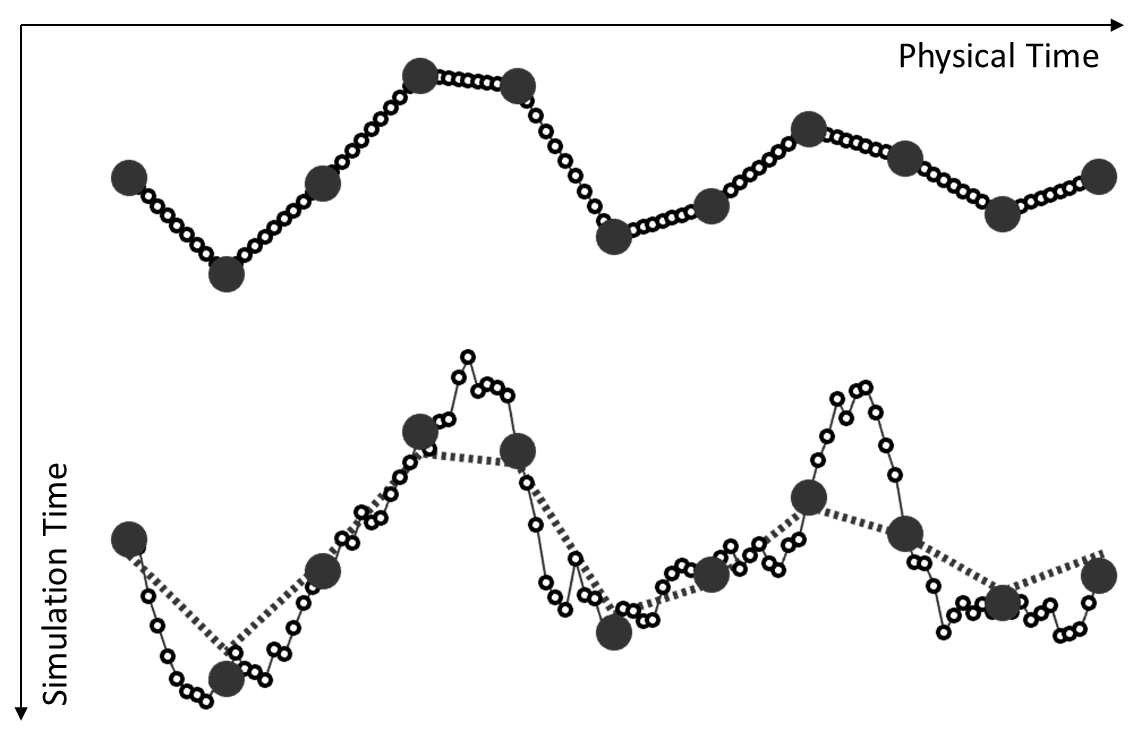
\includegraphics[width=0.7\textwidth]{Figs/FigPolymer.png}
    \caption{Simulated dynamics of a polymer chain with $n+1=11$ data points (large filled circles) and $j-1=9$ intermediate beads (small empty circles). All other parameters are discussed in Section~\ref{numerical_results}. Top: initial state. The intermediate beads represent a linear interpolation to the data points. Bottom: polymer configuration after 1000 iterations of the propagation algorithm. The dotted line represents the initial configuration. It is evident that the new configuration is mostly determined by the dynamics of the low-mass intermediate beads, while the heavy-mass data points barely move from their initial positions.}
    \label{fig:polymer}
\end{figure}

The potential (\ref{Vdisc}) contains terms with different scaling in the potentially large numbers $N$ and $n$, which describe dynamics on different time-scales.
In particular, for large $N$, $V(q,\bt)$ is dominated by its harmonic part and a brute force numerical integration of Hamilton's equations in step (ii) of the HMC algorithm would require a very small discretization time-step to sufficiently resolve its dynamics.
An interesting approximative approach would be to employ a partial averaging of the fast Fourier modes as described in \cite{doll_1985_fourier}.
We choose an exact approach and employ a multiple time scale integration based on Trotter's formula \cite{tuckerman_1993}.

For this purpose it proves to be useful to introduce so-called \emph{staging} variables \cite{tuckerman_1992}, and diagonalize the harmonic part in between the measurement points.
Therefore, we rewrite the discretized harmonic part of the action as
\begin{eqnarray}
  \sum_{i=2}^{N}
  \frac{T}{2\Delta t}
  (q_i-q_{i-1})^2 \nonumber
  \\ =
  \frac{T}{2}
  \sum_{s=1}^{n}\left\{
    \frac{(q_{(s-1)j+1} - q_{sj+1})^2}{j\Delta t}
    +
    \sum_{k=2}^j
    \frac{k}{(k-1)\Delta t}
    (q_{(s-1)j+k}-q^*_{(s-1)j+k})^2
  \right\}\,,\nonumber
  \\
\end{eqnarray}
with
\begin{equation}
  q^*_{(s-1)j+k}
  =
  \frac{(k-1)q_{(s-1)j+k+1} + q_{(s-1)j+1} }{k}
  \,.
\end{equation}
We apply the coordinate transformations
\begin{equation}
  u_{sj+1} = q_{sj+1}\,, \qquad\qquad s=0,\dots,n\, ,
\end{equation}
for the boundary beads, corresponding to the original measurement points, and
\begin{equation}
  u_{sj+k} = q_{sj+k} - q^*_{sj+k}\,, \quad s=0,\dots,n-1\, , \quad k=2,\dots,j\, ,
\end{equation}
for the intermediate staging beads.
The inverse transformations are given by
\begin{eqnarray}
  q_{sj+1} = u_{sj+1}\,,
  \\
  q_{sj+k} = \sum_{l=k}^{j+1}\frac{k-1}{l-1}u_{sj+l}
  +\frac{j-k+1}{j}u_{sj+1}\,.
\end{eqnarray}
The latter can be equivalently expressed by the recursive relation
\begin{equation}
  q_{sj+k} = u_{sj+k} + \frac{k-1}{k} q_{sj+k+1}+ \frac{1}{k}u_{sj+1} \,.
\end{equation}


We split the Hamiltonian $\mathcal{H}_{\mbox{\tiny HMC}}$ into components with different scaling behaviour in the potentially large numbers $n$ and $N$ and write
\begin{equation}
  \mathcal{H}_{\mbox{\tiny HMC}}= \mathcal H_N+\mathcal H_n+\mathcal H_1\,,
\end{equation}
where
\begin{eqnarray}
  \mathcal H_N =
  \frac{1}{2}
  \sum_{s=1}^{n}
  \sum_{k=2}^j
  \left\{
    \frac{\Delta t}{m_q}p_{(s-1)j+k}^2
    +
    \frac{Tk}{\Delta t(k-1)}
    u_{(s-1)j+k}^2
  \right\}\,,\label{H_N}
  \\
  \mathcal H_n =
  \frac{1}{2}
  \sum_{s=1}^{n+1}
  \left\{
   \frac{\Delta t }{m_q}p_{(s-1)j+1}^2
    +
    \frac{(\ln(y_s/r_{(s-1)j+1}) - {\beta u_{(s-1)j+1}})^2}{\sigma^2}
   \right\} \nonumber
   \\
  +
  \frac{T}{2j\Delta t}
  \sum_{s=1}^{n}
    (u_{(s-1)j+1} - u_{sj+1})^2
   \,, \label{H_n} \\
  \mathcal H_1=
   \sum_{\alpha=1}^2\frac{\pi_\alpha^2}{2m_\alpha}
   +
  \frac{\Delta t}{T}
   \sum_{i=2}^{N}
   \left\{
    \frac{1}{2}
     \left(
        \rho_i-\frac{\beta}{\gamma}e^{-\beta q_i}
     \right)^2
    -
    \frac{\beta^2}{2\gamma}
    e^{-\beta q_i}
   -
    T q_i\dot\rho_i
   \right\} \nonumber
  \\
  +
  \frac{1}{\gamma}
  e^{-\beta q_N}
  +
  q_N \rho_{N}
  -
  \frac{1}{\gamma}
  e^{-\beta q_1}
  -
  q_1 \rho_{1} \,. \label{H_1}
\end{eqnarray}
The harmonic part for the staging beads given in Eq.~(\ref{H_N}) scales linearly with $N$. The terms of Eq.~(\ref{H_n}), including both the harmonic part for the boundary beads and the measurement term, scale linearly with $n$. Finally, Eq.~(\ref{H_1}) does not scale with neither $n$ nor $N$.
Thanks to the staging variables $\mathcal H_N$ decouples completely from $\mathcal H_n$.

We use the Trotter formula according to \cite{tuckerman_1992} in order to design a reversible molecular dynamics integrator that takes these different time scales into account.
In order to design an appropriate partition of the Hamiltonian, we need to distinguish different regimes, such as
\begin{enumerate}
  \item[\it i.]
  $\mathcal H_N \sim \mathcal H_n >> \mathcal H_1$,
  \item[\it ii.]
  $\mathcal H_N >> \mathcal H_n \sim \mathcal H_1$,
  \item[\it iii.]
  $\mathcal H_N >> \mathcal H_n >> \mathcal H_1$.
\end{enumerate}
Here, we restrict ourselves to regime ($ii$), i.e., we assume that the number of measurements $n$ is small and/or the measurement error $\sigma$ is large.
The generalization of the method to the other schemes is straightforward.
In regime ($ii$) we simply separate the harmonic part of the action, for the staging beads, from the rest and write
\begin{equation}
  \mathcal{H}_{\mbox{\tiny HMC}}=\mathcal H_N + \mathcal H'\,.
\end{equation}
In order to design a reversible integrator for the associated Hamilton equations, we define the Liouville operators
\begin{equation}
  iL_N=\{\cdot\,,\,\mathcal H_N\}\,,\quad
  iL'=\{\cdot\,,\,\mathcal H'\}\,,
\end{equation}
where $\{\cdot\,,\,\cdot\}$ denotes the Poisson brackets that are defined on functions on the phase space.
Trotter's formula \cite{trotter_1959} allows us to write the Hamiltonian propagator as
\begin{equation}\label{propagator}
  e^{i(L_N+L')\tau}
  =
  (e^{iL_N(\Delta\tau/2)}e^{iL'\Delta\tau}e^{iL_N(\Delta\tau/2)})^P
  +
  \mathcal O(\tau^3/P^{2})\,,
\end{equation}
for $\tau =P\Delta \tau$.
In regime ($ii$) the outer propagator $\exp[iL_N(\Delta \tau/2)]$ describes much faster dynamics than the inner one. However, it is the dynamics of uncoupled harmonic oscillators, which we can readily solve.
Masses and frequencies of the oscillators are derived from (\ref{H_N}) as
\begin{equation}
  m=m_q/\Delta t\,,\quad
  \omega_k=\sqrt{\frac{Nk}{(k-1)m}}\,.
\end{equation}
The fast outer propagator is then given by the equations,
\begin{eqnarray}
  u_{(s-1)j+k}(\Delta\tau/2) \nonumber \\
  = u_{(s-1)j+k}(0)\cos(\omega_k\Delta\tau/2)
  +
  \frac{p_{(s-1)j+k}(0)}{m\omega_k}\sin(\omega_k\Delta\tau/2)\,,\\
  p_{(s-1)j+k}(\Delta\tau/2) \nonumber \\
  = p_{(s-1)j+k}(0)\cos(\omega_k\Delta\tau/2)
  -
  m\omega_k u_{(s-1)j+k}(0) \sin(\omega_k\Delta\tau/2)\,,
\end{eqnarray}
for $s=1,\dots,n$ and $k=2,\dots,j$.

For the inner, slow propagator, we employ the velocity Verlet algorithm \cite{swope_1982_verlet}.
For the boundary beads, it reads
\begin{eqnarray}
  u_{(s-1)j+1}(\Delta\tau) \nonumber \\
  = u_{(s-1)j+1}(0)
  +
  \frac{\Delta\tau}{m} p_{(s-1)j+1}(0)
  +
  \frac{\Delta \tau^2}{2m}
  F_{(s-1)j+1}[\vc u(0),{\pmb\theta}(0)]\,,\\
  p_{(s-1)j+1}(\Delta\tau) \nonumber \\
  = p_{(s-1)j+1}(0)
  +
  \frac{\Delta\tau}{2}
  (
  F_{(s-1)j+1}[\vc u(0),{\pmb\theta}(0)]
  +
  F_{(s-1)j+1}[\vc u(\Delta\tau),{\pmb\theta}(\Delta\tau)]
  )\,,
\end{eqnarray}
with $s=1,\dots,n+1$ and where $F_i[\vc u,{\pmb\theta}]$ denotes the partial derivative of $\mathcal H'[\vc u,{\pmb\theta}]$ w.r.t. $u_i$.
For the model parameters $\bt$ and their momenta ${\pmb\pi}$, analogous equations apply.
When it comes to the staging beads, however, only the momenta have to be updated, because the associated kinetic term is not part of $\mathcal H'$ but of $\mathcal H_N$.
Thus,
\begin{eqnarray}
  p_{(s-1)j+k}(\Delta\tau) \nonumber \\
  =
  p_{(s-1)j+k}(0)
  +
  \frac{\Delta\tau}{2}
  (
  F_{(s-1)j+k}[\vc u(0),{\pmb\theta}(0)]
  +
  F_{(s-1)j+k}[\vc u(\Delta\tau),{\pmb\theta}(\Delta\tau)]
  )
  \,,
\end{eqnarray}
with $s=1,\dots,n$ and $k=2,\dots,j$. The above propagators are applied sequentially $P$ times to calculate the system evolution over the time $\tau$.



\section{Numerical Results}\label{numerical_results}

The algorithm described above was implemented using the free and open-source programming language \emph{Julia} (version 0.3.9)~\cite{julia_web}. One of the attractive features of the language is its (fast growing) library of over 600 packages for numerical and scientific applications.
In our case, we made extensive use of the \emph{ReverseDiffSource} package, which provides a powerful tool for reverse-mode automated differentiation (AD) of arbitrarily complex user-defined expressions. Our algorithm benefits greatly from the use of AD. Indeed, it gives us the possibility to modify the model of eq.~(\ref{sde}) and therefore the action~(\ref{action}) leaving the implementation of the algorithm unaltered. This clearly gives our program significant flexibility making it suitable for a much broader range of applications than the simple exemplary SDE model described here.

We have run preliminary simulations on a 64-bit laptop computer equipped with a Windows 7 operating system, a double-core 1.6~GHz CPU (Intel i5-4200U) and 8~GB of RAM. We have initially used a serial implementation of the algorithm. We assumed $n+1 = 11$ measurement points and $j = 10, 20,\dots, 50$ intermediate staging beads, with a total number of discretization points $N = 101, 201, \dots, 501$. We have set $\Delta\tau = 0.25$ (arbitrary units of time) and $P = 3$ in the Hamiltonian propagator~(\ref{propagator}), with a constant total observation time $T = 833$ (arbitrary units of time). The "true" values of the parameters to be inferred were set to $K_{\mbox{\small true}}=50$~(arbitrary units of time) and $\gamma_{\mbox{\small true}} = 0.2$. Their initial values in our simulations were set to $K=200$~(arbitrary units of time) and $\gamma = 0.5$.

The results shown here were obtained assuming a simple sinusoidal input $r(t) = \sin^2 \left( 0.01 t \right) + 0.1$.
A system realization was first obtained from eq.~(\ref{sde}) using $K_{\mbox{\small true}}$ and $\gamma_{\mbox{\small true}}$. Such system realization was then used to generate a synthetic time series of observed data according to eq.~(\ref{data}). The error $\sigma$ was set to $0.1$.
The input signal, the "true" system realization and the data time series are shown in Fig.~(\ref{fig:rain_data_S})

\begin{figure}[htb!]
    \centering
    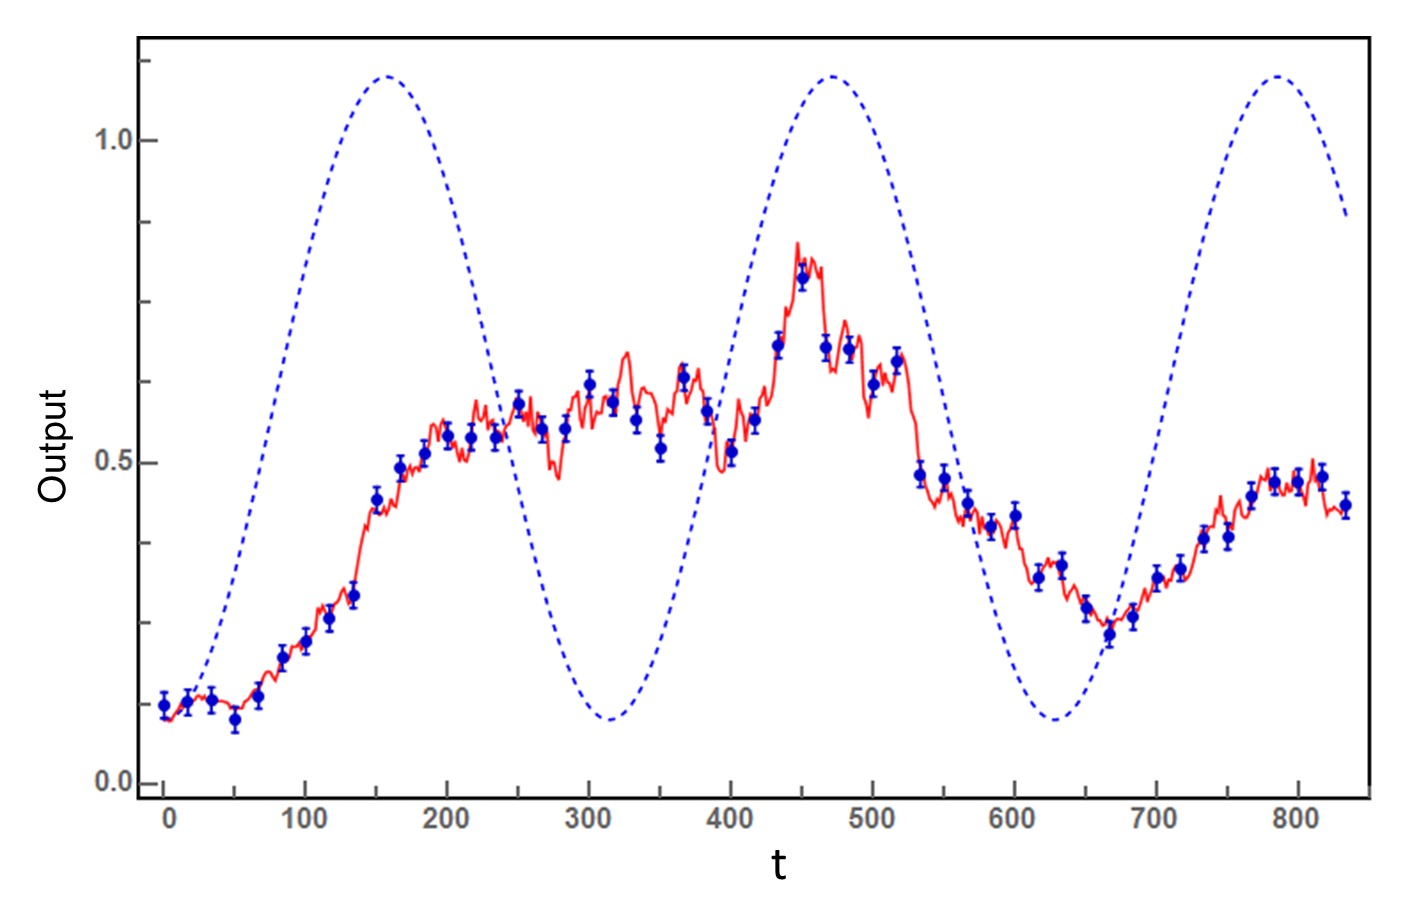
\includegraphics[width=0.6\textwidth]{Figs/FigRainData.png}
    \caption{\label{fig:rain_data_S}Sinusoidal input $r(t)$ (dashed line), "true" system realization with parameters $K_{\mbox{\small true}} = 50$ and $\gamma_{\mbox{\small true}} = 0.2$ (solid line) and synthetic observed data. One may notice how the system response follows the oscillations of the input signal.}
\end{figure}

We observed a reasonably linear dependence of the total computing time on the number of discretization points $N$. In a typical case with $j=30$ (i.e., $N = 301$ discretization points) a complete run with 20000 iterations required about 13 minutes. A set of 200 simulated system realizations is shown in Fig.~(\ref{fig:spaghetti}) together with the synthetic data generated as described above. In the simulation the masses were set to 720 for the boundary beads, 130 for the staging beads and 150 for both the dimensionless parameters $\beta$ and $\gamma$. The different dynamics of the heavy boundary beads and the light staging beads can be appreciated in Fig.~(\ref{fig:spaghetti}).

\begin{figure}[htb!]
    \centering
    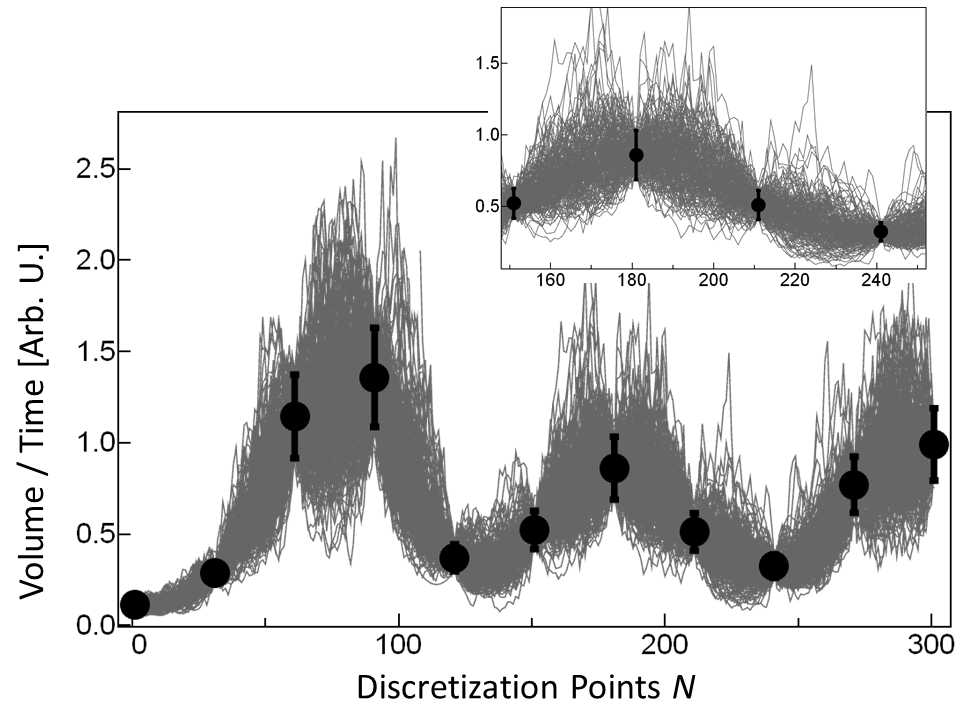
\includegraphics[width=0.7\textwidth]{Figs/FigSpaghetti.png}
    \caption{Simulated system realizations and corresponding synthetic data generated as described in the text. In the inset one may appreciate the different dynamics of heavy data-point and light staging beads.}
    \label{fig:spaghetti}
\end{figure}

\begin{figure}[htb!]
    \centering
    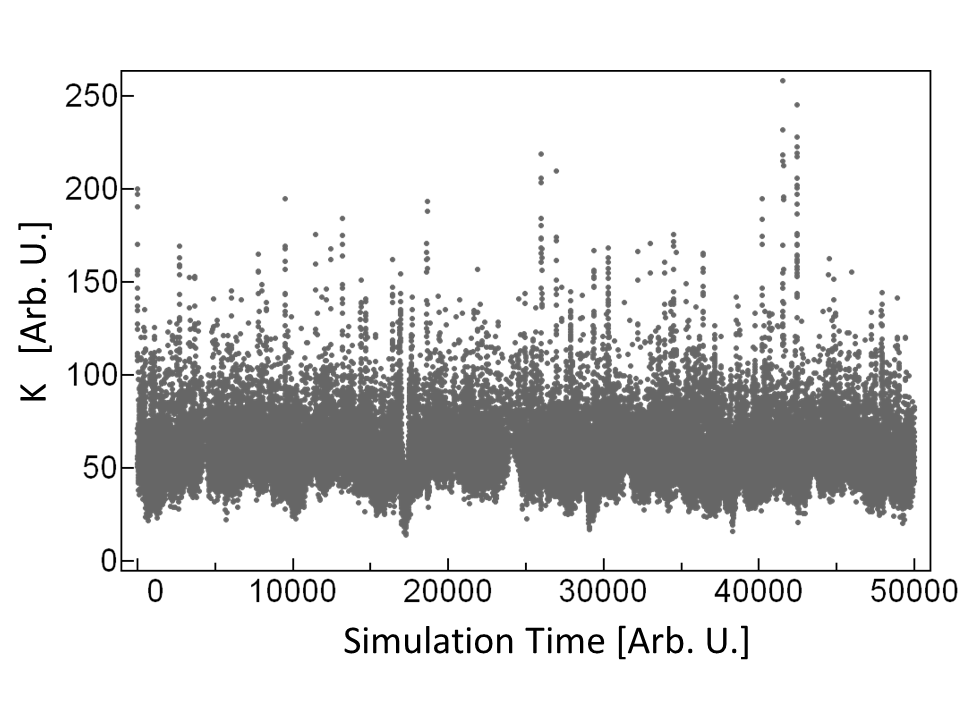
\includegraphics[width=0.7\textwidth]{Figs/FigChainK.png}
    \caption{Markov chain for the inferred parameter $K$.}
    \label{fig:chainK}
\end{figure}

\begin{figure}[htb!]
    \centering
    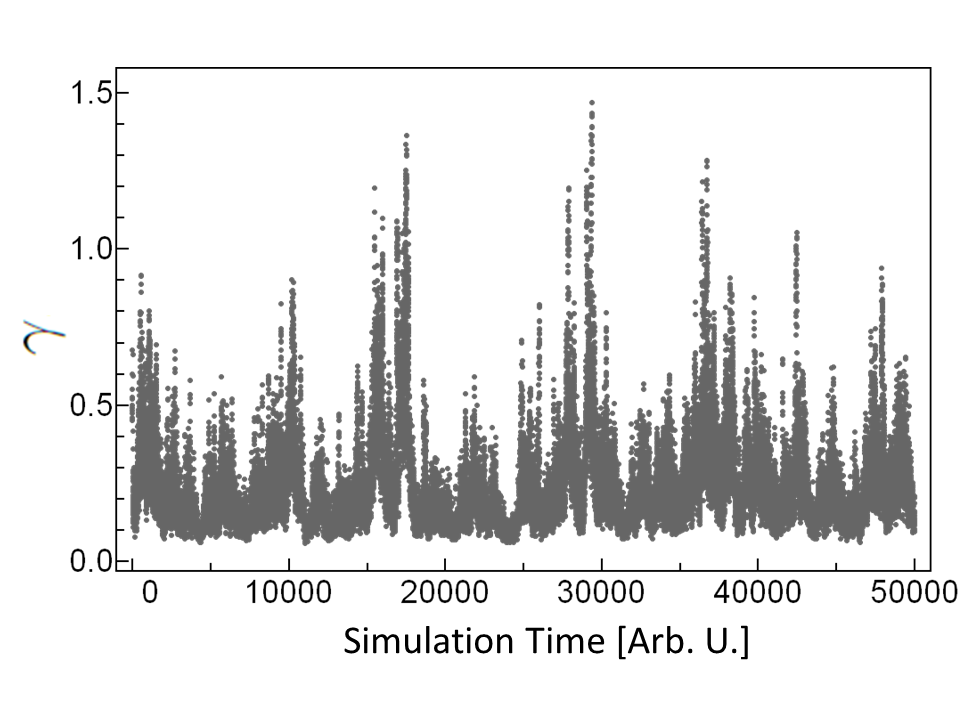
\includegraphics[width=0.7\textwidth]{Figs/FigChainG.png}
    \caption{Markov chain for the inferred parameter $\gamma$.}
    \label{fig:chainG}
\end{figure}

The Markov chains for 50000 iterations for the parameters $K$ and $\gamma$ are shown in Figs.~(\ref{fig:chainK}) and (\ref{fig:chainG}), respectively. Both of them are clearly compatible with the parameter values $K_{\mbox{\small true}} = 50$~(arbitrary units of time) and $\gamma_{\mbox{\small true}} = 0.2$. The system evolution in phase space $K-\gamma$ is shown in Fig.~(\ref{fig:phase_space_evol}). 


%\begin{figure}[htb!]
%    \centering
%    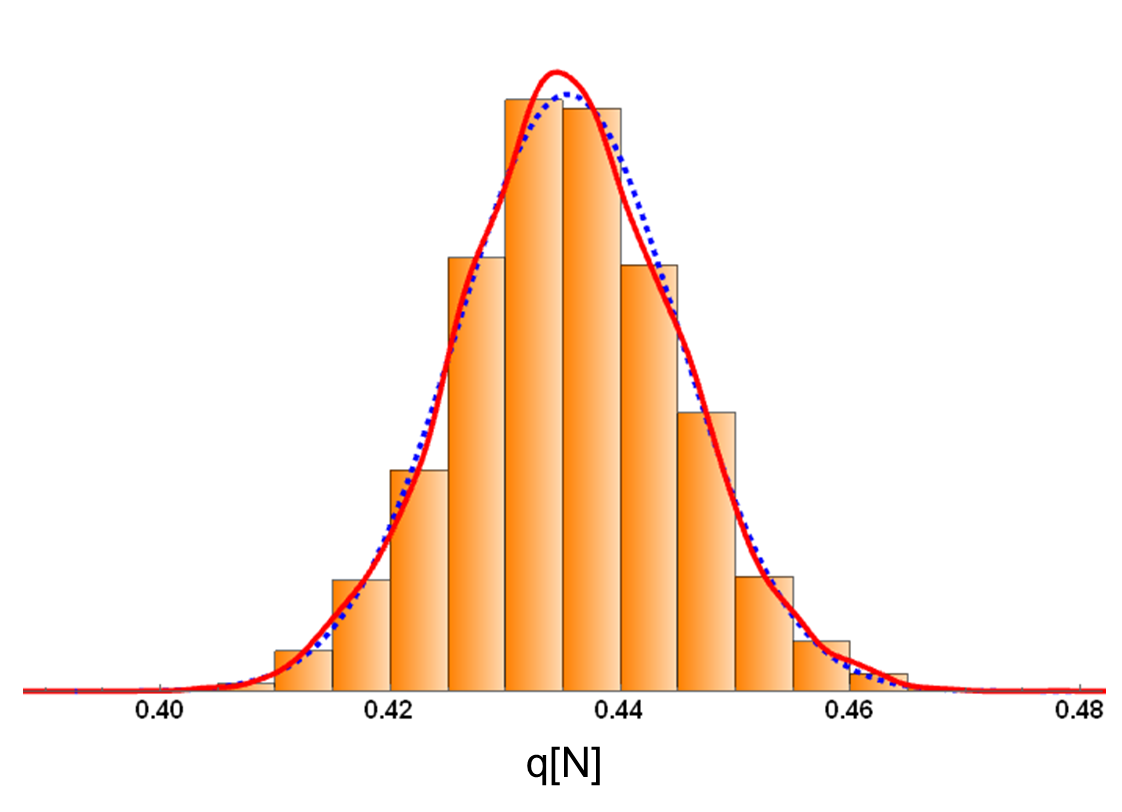
\includegraphics[width=0.3\textwidth]{Figs/FigFinalState.png}
%    \caption{PDF for the system final state expressed via the coordinate set $\left\{ q_N \right\}$. The dashed curve represents a normal distribution with the same mean and variance. The final state is basically normally distributed.}
%    \label{fig:final_state}
%\end{figure}

\begin{figure}[htb!]
    \centering
    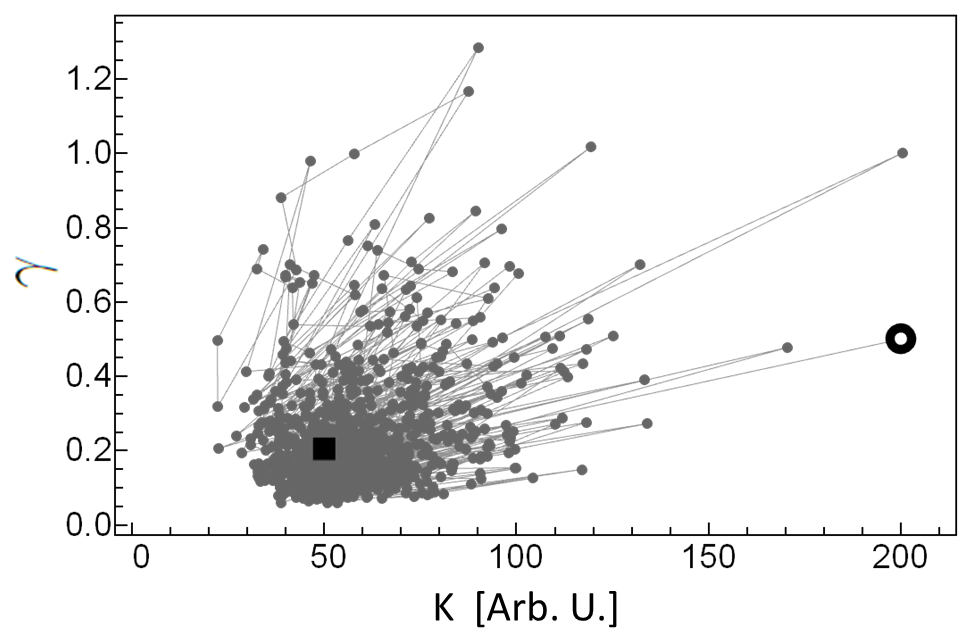
\includegraphics[width=0.7\textwidth]{Figs/FigPhaseSpaceEvol.png}
    \caption{System dynamics in the phase space $K-\gamma$. The empty circle is the initial state, while the square corresponds to the true parameter values used to generate the data.}
    \label{fig:phase_space_evol}
\end{figure}

%\begin{figure}[htb!]
%    \centering
%    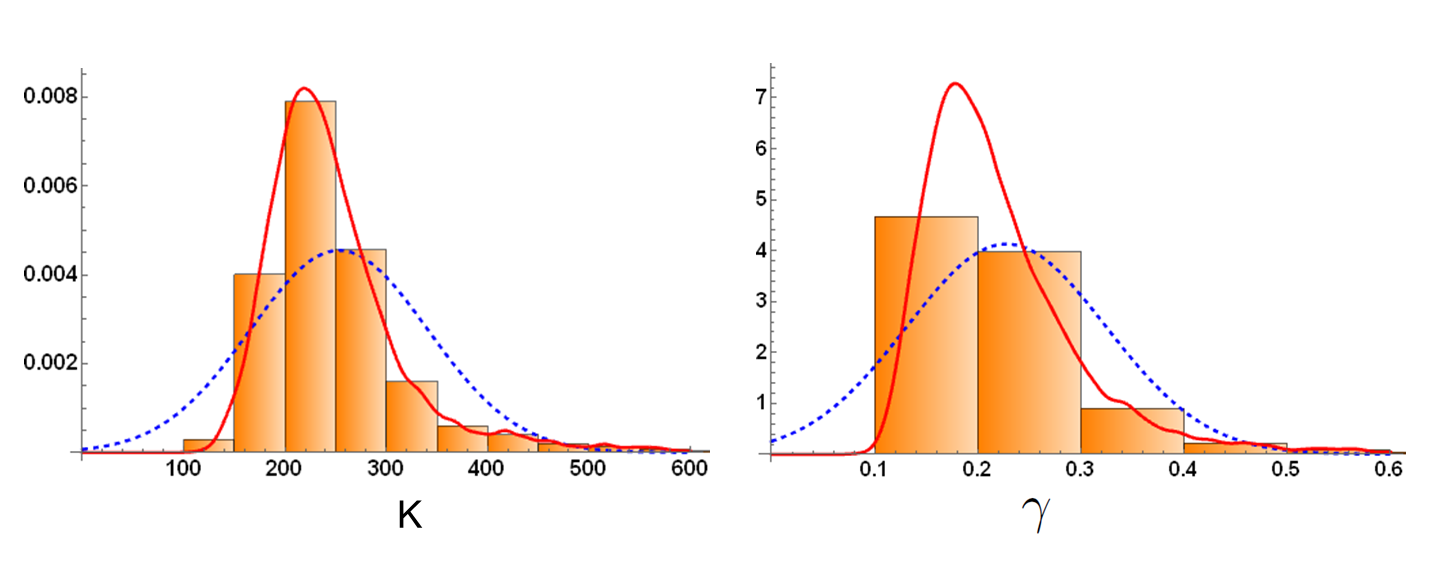
\includegraphics[width=0.5\textwidth]{Figs/FigKg.png}
%    \caption{PDF for the parameters $K$ (left) and $\gamma$ (right). The true values used to generate the data are $K=200$ and $\gamma = 0.2$. The initial values used in the simulations were $K=50$ and $\gamma = 0.4$.}
%    \label{fig:K_distr}
%\end{figure}

\section{Conclusions}

We've presented a new algorithm, for the generation of posterior parameter samples, for ordinary 1D SDE models that are calibrated to time-series.
The algorithm is derived from a re-interpretation of the posterior distribution as a partition function of a 1D statistical mechanical system and employs a Hamiltonian Monte Carlo approach combined with a multiple time-scale integration.
Furthermore, a generic re-parametrization is suggested, which decouples harmonic modes in between measurement points from both the measurement potential and the model parameters, and allows for an efficient analytical integration of these modes.
The algorithm can be implemented in an efficient and generic fashion using automated differentiation and parallelization.
Furthermore, it can easily be adapted to other inference problems.
In particular, it can be adapted to higher dimensional SDEs and SDEs coupled to ODEs.
We explore these adaptations in our future work.

\section*{References}
\bibliographystyle{unsrt}
\bibliography{refs}


\end{document}

